
\section{Lines and Planes in Space} \label{S:9.5.Lines_Planes}

\vspace*{-14 pt}
\framebox{\hspace*{3 pt}
\parbox{6.25 in}{\begin{goals}
\item How are lines in $\R^3$ similar to and different from lines in $\R^2$?
\item What is the role that vectors play in representing equations of lines, particularly in $\R^3$?
\item How can we think of a plane as a set of points determined by a point and a vector?
\item How do we find the equation of a plane through three given non-collinear points?
\end{goals}} \hspace*{3 pt}}

\subsection*{Introduction}

In single variable calculus, we learn that a differentiable function
is \emph{locally linear} \index{locally linear}. In other words, if we
zoom in on the graph of a differentiable function at a point, the
graph looks like the tangent line to the function at that point.  In
multivariable calculus, we will soon study curves in space;
differentiable curves turn out to be locally linear as well.  In
addition, as we study functions of two variables, we will see that
such a function is locally linear at a point if the surface defined by
the function looks like a plane (the tangent plane) as we zoom in on
the graph.

Consequently, it is important for us to understand both lines and
planes in space.  We begin our work by considering some familiar ideas
in $\R^2$ but from a new perspective.

\begin{pa} \label{PA:9.5}
We are familiar with equations of lines in the plane in the form $y = mx+b$, where $m$ is the slope of the line and $(0,b)$ is the $y$-intercept. In this activity, we explore a more flexible way of representing lines that we can use not only in the plane, but in higher dimensions as well.

To begin, consider the line through the point $(2,-1)$ with slope $\frac{2}{3}$.

\begin{figure}[ht]
  \begin{center}
    \includegraphics{fig_9_5_PA1.eps}
  \end{center}
\end{figure}
    \ba
      \item Suppose we increase $x$ by 1 from the point $(2,-1)$. How does the $y$-value change? What is the point on the line with $x$-coordinate $3$?

        \item Suppose we decrease $x$ by 3.25 from the point $(2,-1)$. How does the $y$-value change? What is the point on the line with $x$-coordinate $-1.25$?

        \item Now, suppose we increase $x$ by some arbitrary value $3t$ from the point $(2,-1)$. How does the $y$-value change? What is the point on the line with $x$-coordinate $2+3t$?


        \item Observe that the slope of the line is related to any vector whose $y$-component divided by the $x$-component is the slope of the line. For the line in this exercise, we might use the vector $\langle 3,2 \rangle$, which describes the direction of the line. Explain why the terminal points of the vectors $\vr(t)$, where
             \[\vr(t) = \langle 2,-1 \rangle + \langle 3,2 \rangle t, \]
             trace out the graph of the line through the point $(2,-1)$ with slope $\frac{2}{3}$.


    \item Now we extend this vector approach to $\R^3$ and consider a second example. Let $\mathcal{L}$ be the line in $\R^3$ through the point $(1,0,2)$ in the direction of the vector $\langle 2, -1, 4 \rangle$.

  Find the coordinates of three distinct points on line $\mathcal{L}$. Explain your thinking.


        \item Find a vector in form
        $$\vr(t) = \langle x_0, y_0, z_0 \rangle + \langle a,b,c \rangle t$$ whose terminal points trace out the line $\mathcal{L}$ that is described in (e).  That is, you should be able to locate any point on the line by determining a corresponding value of $t$.
        

    \ea

\end{pa} 



\begin{activitySolution}
    \ba
      \item The slope tells us how the $y$ values change for every unit increase in $x$. So if $x$ increases by 1 from the point $(2,-1)$, the $y$ value increases by $\frac{2}{3}$ to $-\frac{1}{3}$. The point on the line with $x$-coordinate $3$ is then $\left(3,-\frac{1}{3}\right)$.

        \item If $x$ changes by an amount $\Delta x$, then the corresponding change in $y$ is $\frac{\Delta y}{\Delta x} \Delta x$, where $\frac{\Delta y}{\Delta x}$ is the slope of the line. So if $x$ decreases by 3.25 from the point $(2,-1)$, then $y$ changes by ${\frac{2}{3}(-3.25) = -\frac{13}{6}}$. The corresponding point on the line is $\left(-1.25, -\frac{19}{6}\right)$.


        \item If $x$ changes by an amount $3t$, then the corresponding change in $y$ is $\frac{2}{3}(3t) = 2t$. So the new point on the line is ${(x,y) = (2+3t, -1+2t)}$.


        \item We saw in the previous part that an arbitrary point on this line has the form $(2+3t, -1+2t)$. If we think of these points as the terminal points of vectors $\vr(t)$, then we have
\[\vr(t) = \langle 2+3t, -1+2t \rangle =\langle 2,-1 \rangle + \langle 3,2 \rangle t.\]
So the terminal points of the vectors $\vr(t)$ trace out the graph of the line through the point $(2,-1)$ with slope $\frac{2}{3}$.


    \item The point $(1,0,2)$ is given as one point on the line. If we start at the point $(1,0,2)$ and move along the line one step in the direction of the vector $\langle 2, -1, 4 \rangle$, we will arrive at the point
 \[(1+2, 0+(-1), 2+4) = (3,-1,6).\]
Similarly, if we move two steps in the direction of the vector $\langle 2, -1, 4 \rangle$, we will arrive at the point
\[(1+4, 0+(-2), 2+8) = (5,-2,10).\]


        \item Starting at the point $(1,0,2)$ and moving along the line $t$ steps in the direction of the vector $\langle 2, -1, 4 \rangle$, we will arrive at the point
\[(1+2t, 0+(-t), 2+4t).\]
If we consider these points as the terminal points of vectors, we can describe the line as the set of terminal points of the vectors
\[\vr(t) = \langle 1,0,2 \rangle + \langle 2,-1,4\rangle t.\]


    \ea


\end{activitySolution}

\afterpa 

\subsection*{Lines in Space}
In two-dimensional space, a non-vertical line is defined to be the set
of points satisfying the equation
\[y = mx + b,\] for some constants $m$ and $b$. The value of $m$ (the
slope) tells us how the dependent variable changes for every one unit
increase in the independent variable, while the point $(0,b)$ is the
$y$-intercept and anchors the line to a location on the
$y$-axis. Alternatively, we can think of the slope as being related to
the vector $\langle 1, m \rangle$, which tells us the direction of the
line, as shown on the left in Figure \ref{F:9.5.line}. Thus, we can
identify a line in space by fixing a point $P$ and  
a direction $\vv$, as shown on the right.

\begin{figure}[ht]
  \begin{center}
    \includegraphics{figures/fig_9_5_line_slope.eps}
    \caption{A vector description of a line}
    \label{F:9.5.line}
  \end{center}
\end{figure}

\vspace*{5pt}
\nin \framebox{\hspace*{3 pt}
  \parbox{6.25 in}{\begin{definition} \label{D:LineInSpace} A
      \textbf{line}\index{line!in space} in space is the set of
      terminal points of vectors emanating from a given point $P$ that are
      parallel to a fixed vector $\vv$. \end{definition} } \hspace*{3 pt}}
\vspace*{5pt}

The fixed vector $\vv$ in the definition is called a
\emph{direction vector}\index{line!direction vector} for the line. As
we saw in Preview Activity~\ref{PA:9.5}, to find an equation for a
line through point $P$ in the direction of vector $\vv$, observe that
any vector parallel to $\vv$ will have the form $t \vv$ for some
scalar $t$. So, any vector emanating from the point $P$ in a direction
parallel to the vector $\vv$ will be of the form
\begin{equation} \label{eq:9.5.lines_1}
\overrightarrow{OP} + \vv t
\end{equation}
for some scalar $t$ (where $O$ is the origin).

\begin{figure}[ht]
\begin{center}
%\begin{minipage}{2.5in}
%\begin{center}
%\resizebox{!}{2.4in}{\animategraphics[controls]{4}{9_5_L2_}{01}{10}}
\resizebox{!}{1.25in}{\includegraphics{figures/fig_9_5_line_2d_01.eps}} \hspace{0.25in} \resizebox{!}{1.25in}{\includegraphics{figures/fig_9_5_line_2d_10.eps}} \hspace{0.25in} \resizebox{!}{1.25in}{\includegraphics{figures/fig_9_5_line_2d_20.eps}}  
%\animategraphics[controls]{4}{figures/fig_9_5_line_2d_}{00}{25}
%\end{center}
\caption{A line in 2-space.}
\label{F:9.5.Line_2D}
%\end{minipage} \hspace{0.5in}
%\begin{minipage}{2.5in}
%\begin{center}
%\resizebox{!}{2.4in}{\animategraphics[controls,trim=0.5cm 1.5cm 2.5cm 0.5cm]{4}{9_5_L3_}{01}{10}}
%\animategraphics[controls]{4}{figures/fig_9_5_line_3d_}{00}{25}
%\end{center}
%\caption{A line in 3-space.}
%\label{F:9.5.Line_3D}
%\end{minipage}
\end{center}
\end{figure}


Figure \ref{F:9.5.Line_2D} presents three images of a line in two-space in which we can identify the vector
$\overrightarrow{OP}$ and the vector $t \vv$ as in Equation
(\ref{eq:9.5.lines_1}).  Here, $\overrightarrow{OP}$ is the fixed
vector shown in blue, while the direction vector $\vv$ is the vector
parallel to the vector shown in green (that is, the green vector
represents $t\vv$, and the line is traced out by the terminal points
of the magenta vector). In other words, the tips (terminal points) of the magenta vectors (the vectors of the form $\overrightarrow{OP} + t\vv$) trace out the line as $t$ changes. 
%\begin{activity} \label{A:9.5.1} Run the animation in Figure \ref{F:9.5.Line_2D}. Pick a frame and identify the vector $\overrightarrow{OP}$ and the vector $t \vv$ as in equation (\ref{eq:9.5.lines_1}).


\end{activity}
\begin{smallhint}

\end{smallhint}
\begin{bighint}

\end{bighint}
\begin{activitySolution}

\end{activitySolution}
\aftera


In particular, the terminal points of the vectors of the form in
(\ref{eq:9.5.lines_1}) define a linear function $\vr$ in space of the
following form, which is valid in any dimension.

\vspace*{5pt}
\nin \framebox{\hspace*{3 pt}
\parbox{6.25 in}{The \textbf{vector form} of a line\index{line!vector equation} through the point $P$ in the direction of the vector $\vv$ is
\begin{equation} \label{eq:9.5.line_vect}
\vr(t) = \vr_0 + t\vv,
\end{equation}
where $\vr_0$ is the vector $\overrightarrow{OP}$ from the origin to
the point $P$. 
} \hspace*{3 pt}}
\vspace*{5pt}

Of course, it is common to
represent lines in the plane using the slope-intercept equation $y=mx
+ b$.  The vector form of the line, described above, is an
alternative way to represent lines that has the following two
advantages.  First, in two dimensions, we are able to represent
vertical lines, whose slope $m$ is not defined, using a vertical
direction vector, such as $\vv=\langle 0, 1\rangle$.  Second, this
description of lines works in any dimension even though
there is no concept of the slope of a line in more than two dimensions.

\begin{figure}[h]
\begin{center}
%\begin{minipage}{2.5in}
%\begin{center}
%\resizebox{!}{2.4in}{\animategraphics[controls]{4}{9_5_L2_}{01}{10}}
\resizebox{!}{1.25in}{\includegraphics{figures/fig_9_5_line_3d_01.eps}} \hspace{0.25in} \resizebox{!}{1.25in}{\includegraphics{figures/fig_9_5_line_3d_10.eps}} \hspace{0.25in} \resizebox{!}{1.25in}{\includegraphics{figures/fig_9_5_line_3d_20.eps}}  
%\animategraphics[controls]{4}{figures/fig_9_5_line_2d_}{00}{25}
%\end{center}
\caption{A line in 3-space.}
\label{F:9.5.Line_3D}
%\end{minipage} \hspace{0.5in}
%\begin{minipage}{2.5in}
%\begin{center}
%\resizebox{!}{2.4in}{\animategraphics[controls,trim=0.5cm 1.5cm 2.5cm 0.5cm]{4}{9_5_L3_}{01}{10}}
%\animategraphics[controls]{4}{figures/fig_9_5_line_3d_}{00}{25}
%\end{center}
%\caption{A line in 3-space.}
%\label{F:9.5.Line_3D}
%\end{minipage}
\end{center}
\end{figure}

	

\begin{activity} \label{A:9.5.2}  Let $P_1 = (1,2,-1)$ and $P_2 = (-2,1,-2)$. Let $\mathcal{L}$ be the line in $\R^3$ through $P_1$ and $P_2$, and note that three snapshots of this line are shown in Figure \ref{F:9.5.Line_3D}.
	\ba
	\item Find a direction vector for the line $\mathcal{L}$.
	
	\item Find a vector equation of $\mathcal{L}$ in the form $\vr(t) = \vr_0 + t\vv$.
	
	\item Consider the vector equation $\vs(t) = \langle -5, 0, -3 \rangle + t \langle 6, 2, 2 \rangle.$  What is the direction of the line given by $\vs(t)$?  Is this new line parallel to line $\mathcal{L}$?
	
	\item Do $\vr(t)$ and $\vs(t)$ represent the same line, $\mathcal{L}$?  Explain.
	
	\ea


\end{activity}
\begin{smallhint}

\end{smallhint}
\begin{bighint}

\end{bighint}
\begin{activitySolution}
	\ba
	\item Either $\overrightarrow{P_1P_2}$ or $\overrightarrow{P_1P_2}$ will give a direction vector for the line, so one direction vector for the line $\mathcal{L}$ is 
\[\overrightarrow{P_2P_1} = \langle 3, 1, 1 \rangle.\]
	\item We can use the vector $\overrightarrow{OP_1} = \langle 1,2,-1\rangle$ as $\vr_0$, so a vector equation of $\mathcal{L}$ is
\[\vr(t) = \langle 1,2,-1\rangle + t\langle 3, 1, 1 \rangle.\]
	\item The vector $\langle 6, 2, 2 \rangle$ gives the direction of the line determined by $\vs(t)$ Note that $\langle 6, 2, 2 \rangle = 2 \langle 3, 1, 1 \rangle$, so the new line is parallel to line $\mathcal{L}$.
	\item The line $\mathcal{L}$ passes through the point $P_1$. To see if the point $P_1$ also lies on the line with vector representation $\vs(t)$, we need to know if there is a value of $t$ so that 
\begin{equation} \label{eq:Act9.5.2_c_sol}
\langle 1,2,-1\rangle = \langle -5, 0, -3 \rangle + t \langle 6, 2, 2 \rangle.
\end{equation}
If so, then equating the first components shows that $t$ must satisfy the equation $-5+6t=1$. So $t=1$. The second and third components of the  vectors on both sides of equation \ref{eq:Act9.5.2_c_sol} must also be equal when $t=1$. Since $0+2(1) = 2$ and $-3+2(1)=-1$, we see that the point $P_1$ lies on both lines. Since the two lines contain the same point and have the same direction, the lines are the same line. 	
	\ea
\end{activitySolution}
\aftera



\subsection*{The Parametric Equations of a Line}

The vector form of a line, $\vr(t) = \vr_0 + t\vv$ in
Equation~(\ref{eq:9.5.line_vect}), describes a line as the set of
terminal points of the vectors $\vr(t)$. If we write this in terms of
components letting
\[\vr(t) = \langle x(t), y(t), z(t) \rangle, \ \ \ \vr_0 = \langle x_0, y_0, z_0 \rangle, \ \ \ \text{ and } \ \ \ \vv = \langle a, b, c \rangle,\]
then we can equate the components on both sides of $\vr(t) = \vr_0 +
t\vv$ to obtain the equations
\[x(t) = x_0 + at, \ \ \ \ \ y(t) = y_0 + bt, \ \ \ \ \ \text{ and } \ \ \ z(t) = z_0 +
ct,\] which describe the coordinates of the points on the line. The
variable $t$ represents an arbitrary scalar and is called a
\emph{parameter}.  In particular, we use the following language.

\vspace*{5pt}
\nin \framebox{\hspace*{3 pt}
  \parbox{6.25 in}{The \textbf{parametric equations} for a
    line\index{line!parametric equations} through the point $P = (x_0,
    y_0, z_0)$ in the direction of the vector $\vv = \langle a,b,c
    \rangle$ are
\[x(t) = x_0 + at, \ \ \ \ \ y(t) = y_0 + bt, \ \ \ \ \ z(t) = z_0 + ct.\]
} \hspace*{3 pt}}
\vspace*{5pt}

Notice that there are many different parametric equations for the same
line.  For example, choosing another point $P$ on the line or
another direction vector $\vv$ produces another set of parametric
equations.  It is sometimes useful to think of $t$ as a time parameter
and the parametric equations as telling us where we are on the line at
each time.  In this way, the parametric equations describe a
particular walk taken along the line; there are, of course,
many possible ways to walk along a line.

\begin{activity} \label{A:9.5.3}  	Let $P_1 = (1,2,-1)$ and $P_2 = (-2,1,-2)$, and let $\mathcal{L}$ be the line in $\R^3$ through $P_1$ and $P_2$, which is the same line as in Activity \ref{A:9.5.2}.
	\ba
	\item Find parametric equations of the line $\mathcal{L}$.
	
	\item Does the point $(1, 2, 1)$ lie on $\mathcal{L}$? If so, what value of $t$ results in this point?
	
	\item Consider another line, $\mathcal{K}$, whose parametric equations are 
	$$x(s) = -2 + 4s, \ \ y(s) = 1-3s, \ \ z(s) = -2 + 2s.$$
	What is the direction of  line $\mathcal{K}$?
	
	\item Do lines $\mathcal{L}$ and $\mathcal{K}$ intersect?  If so, provide the point of intersection and the $t$ and $s$ values, respectively, that result in the point.  If not, explain why.

	\ea


\end{activity}
\begin{smallhint}

\end{smallhint}
\begin{bighint}

\end{bighint}
\begin{activitySolution}
	\ba
	\item In Activity \ref{A:9.5.2} we saw that a vector form of this line is 
\[\vr(t) = \langle 1,2,-1\rangle + t\langle 3, 1, 1 \rangle.\]
Equating the components give us the following parametric equations for this line: 
\[x(t) = 1 + 3t, \ \ \ y(t) = 2+t, \ \ \ z(t) = -1 + t.\]
	\item To determine if the point $(1, 2, 1)$ lies on $\mathcal{L}$, we need to know if there is a value of $t$ so that 
\[1 = 1 + 3t, \ \ \ 2 = 2+t, \ \ \ 1 = -1 + t.\]
To satisfy the first equation we need to have $t=0$. But then the third equation is not satisfied, so the point  $(1, 2, 1)$ does not lie on $\mathcal{L}$. 
	\item The vector $\langle 4, -3, 2 \rangle$ consisting of the coefficients of the parameter in the parametric equations gives us the direction of the line $\mathcal{K}$.
	\item The direction vectors for the two lines are not scalar multiples of one another, so the lines $\mathcal{L}$ and $\mathcal{K}$ are not parallel and must intersect. The intersection point will occur for values of $s$ and $t$ that simultaneously satisfy the parametric equations of the two lines. In other words, we need to find $s$ and $t$ so that 
\[1+3t = -2+4s, \ \ \ 2+t = 1-3s, \ \ \ \text{ and } \ \ \  -1+t = -2+2s.\]
The second equation gives us $t = -1-3s$. Substituting into the first equation shows that $1+3(-1-3s) = -2+4s$ or $s = 0$. This also implies that $t=-1$. A quick check shows that all three equations are satisfied when $s=0$ and $t=-1$. To find the point of intersection we substitute $t=-1$ into the parametric equations for line $\mathcal{L}$ (or $s=0$ into the parametric equations for line $\mathcal{K}$). We conclude that the two lines intersect at the point $(-2,1,-2)$.  
	\ea

\end{activitySolution}
\aftera
 


% \subsection*{The Symmetric Equations of a Line}

% So far, we have seen that a line can be represented parametrically, where the parameter's value enables us to locate various points along the line as the parameter changes.  In addition, we saw in Activity~\ref{A:9.5.2} that it a given line has more than one parameterization.  Next, we observe that in certain circumstances, we can describe a line in space through a different set of equations that are independent of a parameter.

% In particular, if we assume that $a$, $b$, and $c$ are nonzero in the parametric equations of a given line, then we can solve each of the three equations for $t$ and obtain the \emph{symmetric equations} of the line
% %\[\frac{x-x_0}{a} = \frac{y-y_0}{b} = \frac{z-z_0}{c}.\]
% %If any one of $a$, $b$, or $c$ is 0, then the line is parallel to one of the coordinate planes. For example, if $a=0$ and $b$ and $c$ are %non-zero, then the line is in the plane $x=x_0$ and the symmetric equations for the line are
% %\[\frac{y-y_0}{b} = \frac{z-z_0}{c} \ \text{ and } x = x_0.\]

% \vspace*{5pt}
% \nin \framebox{\hspace*{3 pt}
% \parbox{6.25 in}{The \textbf{symmetric equations} for a line\index{line!symmetric equations} through the point $P = (x_0, y_0, z_0)$ in the direction of the vector $\vv = \langle a,b,c \rangle$ are
% \[\frac{x-x_0}{a} = \frac{y-y_0}{b} = \frac{z-z_0}{c},\]
% provided that $a$, $b$, and $c$ are not zero.
% } \hspace*{3 pt}}
% \vspace*{5pt}

% For example, for the line $\mathcal{L}$ in Activity~\ref{A:9.5.2}, which passes through $P_1 = (1,2,-1)$ and $P_2=(-2,1,-2)$, which has parametric equations
% $$x(t) = 1-3t, \ \ y(t) = 2-t, \ \ z(t) = -1-t,$$
% the symmetric equations are 
% $$\frac{x-1}{-3} = \frac{y-2}{-1} = \frac{z+1}{-1}.$$

% %\begin{activity} \label{A:9.5.4}  	Let $P_1 = (1,2,-1)$ and $P_2 = (-2,1,-2)$, and let $\mathcal{L}$ be the line in $\R^3$ through $P_1$ and $P_2$ as in Activity \ref{A:9.5.2}.
	\ba
	\item Find the symmetric equations of the line $\mathcal{L}$.
	
	
	
	\item What will the symmetric equations look like if $a=0$? Explain.
	
	
	
	\ea


\end{activity}
\begin{smallhint}

\end{smallhint}
\begin{bighint}

\end{bighint}
\begin{activitySolution}

\end{activitySolution}
\aftera

% %\begin{activity} \label{A:9.5.5}  Let $P_1 = (1,2,-1)$ and $P_2 = (-2,1,-2)$, and let $\mathcal{L}$ be the line in $\R^3$ through $P_1$ and $P_2$ as in Activity \ref{A:9.5.2}.
	\ba
	\item What values of the parameter $t$ describe the entire line $\mathcal{L}$?
	
	
	
	\item What value of the parameter $t$ makes $(x(t), y(t), z(t)) = P_1$?
	
	
	
	\item What value of the parameter $t$ makes $(x(t), y(t), z(t)) = P_2$?
	
	
	
	\item What restrictions on the parameter $t$ describe the line segment between the points $P_1$ and $P_2$?
	
	
	
	\ea


\end{activity}
\begin{smallhint}

\end{smallhint}
\begin{bighint}

\end{bighint}
\begin{activitySolution}

\end{activitySolution}
\aftera




\subsection*{Planes in Space}

Now that we have a way of describing lines, we would like to develop a means of describing planes in three dimensions.  We studied the coordinate planes and planes parallel to them in Section \ref{S:9.1.Functions}. Each of those planes had one of the variables $x$, $y$, or $z$ equal to a constant. We can note that any vector in a plane with $x$ constant is orthogonal to the vector $\langle 1,0,0 \rangle$, any vector in a plane with $y$ constant is orthogonal to the vector $\langle 0,1,0 \rangle$, and any vector in a plane with $z$ constant is orthogonal to the vector $\langle 0,0,1 \rangle$.  This idea works in general to define a plane. 

\vspace*{5pt}
\nin \framebox{\hspace*{3 pt}
  \parbox{6.25 in}{\begin{definition} A
      \textbf{plane}\index{plane!definition} $p$ in space is the set of
      all terminal points of vectors emanating from a given point
      $P_0$ perpendicular to a fixed vector $\vn$, as shown in Figure
      \ref{F:9.5.plane.normal}. \end{definition} }
  \hspace*{3 pt}} \vspace*{5pt} 

\begin{figure}[ht]
  \begin{center}
    \includegraphics{figures/fig_9_5_plane_normal.eps}
    \caption{A point $P_0$ on a plane $p$ with a normal vector $\vn$}
    \label{F:9.5.plane.normal}
  \end{center}
\end{figure}

The definition allows us to find the equation of a plane. Assume that $\vn=\langle a,b,c\rangle$, $P_0 =
(x_0, y_0, z_0)$, and that $P=(x,y,z)$ is an arbitrary point on the plane.
Since the vector $\overrightarrow{PP_0}$ lies in
the plane, it must be perpendicular to $\vn$.  This means that

\begin{eqnarray*}
  0 & = & \vn\cdot\overrightarrow{PP_0}  \\
     & = & \vn\cdot \big(\langle x,y,z \rangle - \langle x_0, y_0,
    z_0\rangle\big)  \\
     &=& \vn \cdot \langle x-x_0, y-y_0, z-z_0 \rangle  \\
     &=& a(x-x_0) + b(y-y_0) + c(z-z_0). \\
\end{eqnarray*}

The fixed vector $\vn$ perpendicular to the plane is frequently called
a {\em normal vector} to the plane.  We may now summarize as follows.

\vspace*{5pt}
\nin \framebox{\hspace*{3 pt}
  \parbox{6.25 in}{The \textbf{scalar equation} of the
    plane\index{plane!scalar equation} with normal vector $\vn =
    \langle a,b,c \rangle$ containing the point $P_0 = (x_0, y_0,
    z_0)$ is
\begin{equation}\label{eq:9.5.plane_norm}
a(x-x_0) + b(y-y_0) + c(z-z_0) = 0.
\end{equation}
} \hspace*{3 pt}}
\vspace*{5pt}

We may take this a little further and note that since
\begin{equation*}
  a(x-x_0) + b(y-y_0) + c(z-z_0) = 0, 
\end{equation*}
it equivalently follows that
\begin{equation*}
  ax + by + cz = ax_0+by_0+cz_0.
\end{equation*}
That is, we may write the equation of a plane as $ax+by+cz = d$ where
where $d = \vn\cdot\langle x_0,y_0,z_0\rangle$.  

For instance, if we would like to describe the plane passing through
the point $P_0=(4, -2,1)$ and perpendicular to the vector $\vn =
\langle 1, 2, 1 \rangle$, we have
$$
  \langle 1,2,1 \rangle\cdot \langle x,y,z\rangle =
  \langle 1,2,1 \rangle\cdot \langle 4,-2,1\rangle 
$$
or
$$
x + 2y + z = 1.
$$

Notice that the coefficients of $x$, $y$, and $z$ in this description
give a vector perpendicular to the plane.  For instance, if we are
presented with the plane
$$
-2x + y - 3z = 4,
$$
we know that $\vn = \langle -2, 1, -3\rangle$ is a vector
perpendicular to the plane.
  
\begin{activity} \label{A:9.5.9} 
  \ba
\item Write the equation of the plane $p_1$ passing through the point $(0,
  2, 4)$ and perpendicular to the vector $\vn=\langle 2, -1,
  1\rangle$.

\item Is the point $(2, 0, 2)$ on the plane $p_1$?

\item Write the equation of the plane $p_2$ that is parallel to $p_1$
  and passing through the point $(3, 0, 4)$.  
	
\item Write the parametric description of the line $l$ passing through the
  point $(2,0,2)$ and perpendicular to the plane $p_3$ described the
  equation $x+2y-2z = 7$.

\item Find the point at which $l$ intersects the plane $p_3$.
	
	
	\ea


\end{activity}
\begin{smallhint}

\end{smallhint}
\begin{bighint}

\end{bighint}
\begin{activitySolution}
\ba
\item The plane has equation $2x-(y-2)+(z-4)=0$. 


\item Since $2(2)-(0-2)+(2-4) \neq 0$, the point point $(2, 0, 2)$ is not on the plane $p_1$.

\item Parallel planes will have parallel normal vectors, so an equation of the plane $p_2$ that is parallel to $p_1$
  and passing through the point $(3, 0, 4)$ is $2(x-3)-y+(z-4)=0$.   
	
\item A direction vector for $l$ will be a normal vector for $p_3$, or $\langle 1,2,-2\rangle$. So a parametric description of the line $l$ is 
\[x(t) = 2+t \ \ y(t) = 2t \ \ z(t) = 2-2t.\]

\item When $l$ intersects $p_3$ we will have $(2+t)+2(2t)-2(2-2t) = 7$. This happens when $t=1$, which gives the point of intersection as $(3,2,0)$. 
\ea
\end{activitySolution}
\aftera


Just as two distinct points in space determine a line, three
non-collinear points in space determine a plane.  
% Alternatively, we
% know that for a line, a single point and a direction vector suffice to
% determine the line.  For a plane, we will see that a single point and
% a \emph{normal vector} (that is, a vector perpendicular to the plane)
% will fully characterize the plane.
Consider three points $P_0$, $P_1$, and $P_2$ in space, not all lying
on the same line as shown in Figure \ref{F:9.5.Plane}.
\begin{figure}[ht]
\begin{center}
%\resizebox{!}{1.0in}{\includegraphics{9_5_Plane}}
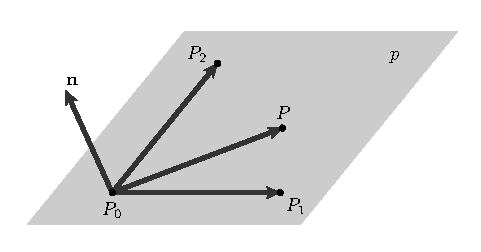
\includegraphics{fig_9_5_plane_3pts.eps}
\end{center}
\caption{A plane determined by three points $P_0$, $P_1$, and $P_2$}
\label{F:9.5.Plane}
\end{figure}
% We would like to find an equation of the plane $p$ that contains these
% points, and thus describes the set of all points on the plane.

Observe that the vectors $\overrightarrow{P_0P_1}$ and
$\overrightarrow{P_0P_2}$ both lie in the plane $p$.  
If we form their cross-product
$$\vn = \overrightarrow{P_0P_1} \times \overrightarrow{P_0P_2},$$
we obtain a normal vector to the plane $p$.  
Therefore, if $P$ is any other point on  $p$, it then follows that
$\overrightarrow{P_0P}$ will be perpendicular to $\vn$, and we have,
as before, the equation
\begin{equation} \label{eq:9.5.plane_vect}
\vn \cdot \overrightarrow{P_0P} = 0.
\end{equation}

%\begin{activity} \label{A:9.5.6}  	Notice that the vectors $\overrightarrow{P_0P_1}$ and $\overrightarrow{P_0P_2}$ both lie in the plane $p$.
    \ba
    \item What vector $\vn$ do we know that is perpendicular to both $\overrightarrow{P_0P_1}$ and $\overrightarrow{P_0P_2}$?



\begin{comment}

The cross product $\vn = \overrightarrow{P_0P_1} \times \overrightarrow{P_0P_2}$ is a vector perpendicular to both $\overrightarrow{P_0P_1}$ and $\overrightarrow{P_0P_2}$.

\end{comment}

    \item Let $P$ be any point the plane $p$. What relationship will the vector $\overrightarrow{P_0P}$ have to $\vn$?



\begin{comment}

In fact, if $P$ is any point in the plane $p$, then the vector $\overrightarrow{P_0P}$ is orthogonal to $\vn$.

\end{comment}

    \item Explain why the equation
\begin{equation}
\overrightarrow{P_0P} \cdot \vn = 0. \label{eq:9.5.plane_vect}
\end{equation}
describes all points in the plane $p$.



    \ea


\end{activity}
\begin{smallhint}

\end{smallhint}
\begin{bighint}

\end{bighint}
\begin{activitySolution}

\end{activitySolution}
\aftera

% Equation (\ref{eq:9.5.plane_vect}) is the \emph{vector form}\index{plane!vector form} of the equation of a plane, and further helps us to naturally characterize a plane. 
% This equation also tells us that a plane is the set of terminal points of vectors from a fixed point that are perpendicular to the vector $\vn$ in \ref{eq:9.5.plane_vect}.

% The fixed vector in the definition of a plane is called a \emph{normal vector}\index{plane!normal vector} to the plane; in Equation~(\ref{eq:9.5.plane_vect}), the vector $\vn$ is a normal vector.  If we let $P_0 = (x_0, y_0, z_0)$ and $\vn = \langle a, b, c \rangle$ be given, and let $P = (x,y,z)$ be an arbitrary point in the plane, then Equation~(\ref{eq:9.5.plane_vect}) tells us that
% $$
% \langle x-x_0, y-y_0, z-z_0 \rangle \cdot \langle a,b,c \rangle = 0.
% $$
% When we expand the dot product in this most recent equation, we get an important standard form of the equation of a plane.

\begin{activity} \label{A:9.5.7}  	Let $P_0 = (1,2,-1)$, $P_1 = (1, 0 ,-1)$, and $P_2 = (0,1,3)$ and let $p$ be the plane containing $P_0$, $P_1$, and $P_2$.
	\ba
	\item Determine the components of the vectors $\overrightarrow{P_0P_1}$ and $\overrightarrow{P_0P_2}$.	
	\item Find a normal vector $\vn$ to the plane $p$.
	\item Find the scalar equation of the plane $p$.
	\item Consider a second plane, $q$, whose scalar equation is $-3(x-1) + 4(y+3) + 2(z-5)=0$.  Find two different points on plane $q$, as well as a vector $\vm$ that is normal to $q$.
	\item We define the angle between two planes to be the angle between their respective normal vectors.  What is the angle between planes $p$ and $q$? 

	\ea


\end{activity}
\begin{smallhint}

\end{smallhint}
\begin{bighint}

\end{bighint}
\begin{activitySolution}
	\ba
	\item A straightforward computation shows that 
\[\overrightarrow{P_0P_1} = \langle 0, -2, 0 \rangle \ \ \ \text{ and } \ \ \ \overrightarrow{P_0P_2} = \langle -1, -1, 4 \rangle.\]	
	\item Since the vectors $\overrightarrow{P_0P_1}$ and $\overrightarrow{P_0P_2}$ lie in the plane, the cross product 
\[\vn = \overrightarrow{P_0P_1} \times \overrightarrow{P_0P_2} = \langle 0, -2, 0 \rangle \times \langle -1, -1, 4 \rangle = \langle 8,0,-2 \rangle\]
is a normal vector $\vn$ to the plane $p$.
	\item Using the point $P_0$, the scalar equation of the plane $p$ is
	\[(-8)(x-1)+(0)(y-2) +(-2)(z+1) = 0\]
	or
	\[8x+2z=6.\]
	\item To find a point on the plane, choose values for $x$ and $y$, and that will determine the corresponding value for $z$. If $x=1$ and $y=-3$, then $z=5$ and the point $(1,-3,5$ lies in the plane $q$. If $x=1$ and $y=-2$, then $z=3$ and the point $(1,-2,3)$ lines in the plane $q$. A normal vector $\vm = \langle -3, 4, 2 \rangle$ to $q$ is the vector of coefficients of $x$, $y$, and $z$ in the scalar equation of the plane. 
	\item The angle $\theta$ between $\vn$ and $\vm$ is found by
\[\theta = \cos^{-1}\left(\frac{\vn \cdot \vm}{|\vn| \ |\vm|} \right) = \cos^{-1}\left(\frac{-28}{\sqrt{68}\sqrt{29}}\right) \approx 129.1^{\circ}.\]
	\ea
\end{activitySolution}
\aftera


%We can use what we know about vectors and projections to find the distance from a point to a plane.

%\begin{activity} \label{A:9.5.8}  Let $p$ be the plane with equation $z=-4x+3y+4$, whose graph is shown in Figure \ref{F:9.5.Point_to_plane}. (Note that we can always find an equation of this form by expanding the scalar equation and collecting the constant terms). Let $Q = (4,-1,8)$.
\begin{figure}[ht]
\begin{center}
\resizebox{!}{2.5in}{\includegraphics[trim=0cm 0.25cm 0cm 1.5cm, clip]{9_5_Point_to_plane}}
\end{center}
\caption{Graph of $z=-4x+3y+4$.}
\label{F:9.5.Point_to_plane}
\end{figure}
%crop graphics in animate trim=<left> <bottom> <right> <top>, add, clip with \includegraphics
	\ba
	\item Show that $Q$ does not lie in the plane $p$.
	
	
	
	\item Find a normal vector $\vn$ to the plane $p$.
	
	
	
	\item Find the coordinates of a point $P$ in $p$.
	


	\item Find the components of $\overrightarrow{PQ}$. Draw a picture in Figure \ref{F:9.5.Point_to_plane} to illustrate the objects found so far.
	
	
	
	\item Explain why $|\comp_{\vn} \overrightarrow{PQ}|$ gives the distance from the point $Q$ to the plane $p$. Find this distance.
	
	
	
	\ea


\end{activity}
\begin{smallhint}

\end{smallhint}
\begin{bighint}

\end{bighint}
\begin{activitySolution}

\end{activitySolution}
\aftera


\begin{summary}
\item While lines in $\R^3$ do not have a slope, like lines in $\R^2$ they can be characterized by a point and a direction vector.  Indeed, we define a line in space to be the set of terminal points of vectors emanating from a given point that are parallel to a fixed vector.
\item Vectors play a critical role in representing the equation of a line.  In particular, the terminal points of the vector $\vr(t) = \vr_0 + t\vv$ define a linear function $\vr$ in space through the terminal point of the vector $\vr_0$ in the direction of the vector $\vv$, tracing out a line in space.
\item A plane in space is the set of all terminal points of vectors emanating from a given point perpendicular to a fixed vector.
\item If $P_1$, $P_2$, and $P_3$ are non-collinear points in space, the vectors $\overrightarrow{P_1P_2}$ and and $\overrightarrow{P_1P_3}$  are vectors in the plane and the vector $\vn = \overrightarrow{P_1P_2} \times \overrightarrow{P_1P_3}$ is a normal vector to the plane. So any point $P$ in the plane satisfies the equation $\overrightarrow{PP_1} \cdot \vn = 0$.  If we let $P = (x,y,z)$, $\vn = \langle a,b,c \rangle$ be the normal vector, and $P_1 = (x_0,y_0,z_0)$, we can also represent the plane with the equation
$$a(x-x_0) + b(y-y_0) + c(z-z_0) = 0.$$
\end{summary}

\nin \hrulefill

\begin{exercises} 

\item \label{Ez:9.5.1}   The vector and parametric forms of a line allow us to easily describe line segments in space. 

Let $P_1 = (1,2,-1)$ and $P_2 = (-2,1,-2)$, and let $\mathcal{L}$ be the line in $\R^3$ through $P_1$ and $P_2$ as in Activity \ref{A:9.5.2}.
\ba
	\item What value of the parameter $t$ makes $(x(t), y(t), z(t)) = P_1$? What value of $t$ makes $(x(t), y(t), z(t)) = P_2$?	
	\item What restrictions on the parameter $t$ describe the line segment between the points $P_1$ and $P_2$?
	\item What about the line segment (along the same line) from $(7,4,1)$ to $(-8,-1,-4)$?
	\item Now, consider a segment that lies on a different line:  parameterize the segment that connects point $R=(4,-2,7)$ to $Q=(-11,4,27)$ in such a way that $t = 0$ corresponds to point $Q$, while $t = 2$ corresponds to $R$.
	\ea
%\begin{figure}[h]
%\begin{center}
 %\includegraphics{figures/1_1_Ez1.eps}
 %\caption{A bungee jumper's height function.} \label{F:1.1.Ez1}
%\end{center}
%\end{figure}

\begin{exerciseSolution}
	\ba
	\item The line $\mathcal{L}$ can be expressed in vector form as $\vr(t) = \langle 1,2,-1\rangle + t\langle -3,-1,-1 \rangle$ and in parametric form as $x(t) = 1-3t$, $y(t) = 2-t$, and $z(t) = -1-t$. Note that $(x(0), y(0), z(0)) = P_1$ and $(x(1), y(1), z(1)) = P_2$. 
	\item If we restrict $t$ to be in the interval $[0,1]$ then our parameterization describes the line segment between the points $P_1$ and $P_2$.
	\item Here we note that $(x(-2), y(-2), z(-2)) = (7,4,1)$ and $(x(3), y(3), z(3)) = (-8,-1,-4)$. So restricting $t$ to lie in the interval $[-2,3]$ the parameterization describes the line segment from $(7,4,1)$ to $(-8,-1,-4)$.
	\item Since we want our parameterization be at $Q$ when $t=0$ and $R$ at $t=2$, we use the vector $\frac{1}{2}\overrightarrow{QR} = \frac{1}{2} \langle 15,-6,-20 \rangle$ as a direction vector for this line. So a parameterization of the segment that connects point $R=(4,-2,7)$ to $Q=(-11,4,27)$ in such a way that $t = 0$ corresponds to point $Q$, while $t = 2$ corresponds to $R$ is $x(t) = -11+\frac{15}{2}t$, $y(t) = 4-3t$, and $z(t) = 27-10t$.
	\ea
\end{exerciseSolution}

\item \label{Ez:9.5.2}   This exercise explores key relationships between a pair of lines.  Consider the following two lines:  one with parametric equations $x(s) = 4-2s$, $y(s) = -2 + s$, $z(s) = 1 + 3s$, and the other being the line through $(-4, 2, 17)$ in the direction $\vv = \langle -2, 1, 5 \rangle$.

%\begin{figure}[h]
%\begin{center}
 %\includegraphics{figures/1_1_Ez1.eps}
 %\caption{A bungee jumper's height function.} \label{F:1.1.Ez1}
%\end{center}
%\end{figure}

  \ba
  	\item  Find a direction vector for the first line, which is given in parametric form.
	\item  Find parametric equations for the second line, written in terms of the parameter $t$.
	\item  Show that the two lines intersect at a single point by finding the values of $s$ and $t$ that result in the same point.
	\item  Find the angle formed where the two lines intersect, noting that this angle will be given by the angle between their respective direction vectors.  
 	\item  Find an equation for the plane that contains both of the lines described in this problem. 
  \ea 


\begin{exerciseSolution}
  \ba
  	\item  The coefficients on the parameter provide a direction vector for the line, so a direction vector for the first line is $\langle -2, 1, 3 \rangle$. 
	\item  We are given a point and a direction, so a set of parametric equations for the second line is $x(t) = -4-2t$, $y(t) = 2+t$, and $z(t) = 17+5t$. 
	\item  A point that lies on both lines must simultaneously satisfy both sets of parametric equations. In other words, there must be a value of $s$ and a value of $t$ so that 
\begin{align*}
4-2s = -4-2t \\
-2 + s &=  2+t \\
1+3s &= 17+5t.
\end{align*}
The first and second equations are the same, both giving $s=t+4$. Substituting for $s$ in the third equation yields $t=-2$ and then $s=2$. This gives the point of intersection of the two lines as $(0,0,7)$. 
	\item  The direction vectors are $\vu = \langle -2, 1, 3 \rangle$ and $\vv = \langle -2, 1, 5 \rangle$. Then angle $\theta$ between $\vu$ and $\vv$ is given by 
\[\theta = \cos^{-1}\left(\frac{\vu \cdot \vv}{|\vu| |\vv|} \right) = \cos^{-1}\left(\frac{20}{\sqrt{14} \sqrt{30}} \right) \approx 12.6^{\circ}.\]
 	\item The plane will contain both direction vectors, so a normal to this plane is 
\[\vu \times \vv = \langle = \langle 2, 4, 0 \rangle.\]
The point $(-4,2,17)$ lies in this plane, so the equation of the plane that contains both lines is 
\[2(x+4)+4(y-2) = 0.\]
  \ea 
\end{exerciseSolution}

\item \label{Ez:9.5.3}   This exercise explores key relationships between a pair of planes.  Consider the following two planes:  one with scalar equation $4x - 5y + z = -2$, and the other which passes through the points $(1,1,1)$, $(0,1,-1)$, and $(4, 2, -1)$.

%\begin{figure}[h]
%\begin{center}
 %\includegraphics{figures/1_1_Ez1.eps}
 %\caption{A bungee jumper's height function.} \label{F:1.1.Ez1}
%\end{center}
%\end{figure}

  \ba
  	\item  Find a vector normal to the first plane.
	\item  Find the scalar equation for the second plane.
	\item  Find the angle between the planes, where the angle between them is defined by the angle between their respective normal vectors.
	\item  Find a point that lies on both planes.
	\item  Since these two planes do not have parallel normal vectors, the planes must intersect, and thus must intersect in a line.  Observe that the line of intersection lies in both planes, and thus the direction vector of the line must be perpendicular to each of the respective normal vectors of the two planes.  Find a direction vector for the line of intersection for the two planes.
	\item  Determine parametric equations for the line of intersection of the two planes. 
  \ea

\begin{exerciseSolution}
  \ba
  	\item  The coefficients of $x$, $y$, and $z$ tell us a normal vector for the first plane, so a normal vector for the first plane is $\langle 4, -5, 1 \rangle$. 
	\item  Let $P = (1,1,1)$, $Q = (0,1,-1)$ and $R = (4,2,-1)$. A normal vector for the plane will be 
\[\overrightarrow{PQ} \times \overrightarrow{PR} = \langle -1,0,-2 \rangle \times \langle 3, 1, -2 \rangle = \langle 2, -8, -1 \rangle.\]
Using the point $P$ gives us the scalar equation 
\[2(x-1) - 8(y-1) - (z-1) = 0.\]
	\item  The normal vectors are $\vn_1 = \langle 4, -5, 1 \rangle$ and $\vn_2 = \langle 2, -8, -1 \rangle$. The angle $\theta$ between the planes is the angle between $\vn_1$ and $\vn_2$ or 
\[\theta = \cos^{-1}\left(\frac{\vn_1 \cdot \vn_2}{|\vn_1| |\vn_2|} \right) = \cos^{-1}\left(\frac{47}{\sqrt{42} \sqrt{69}} \right) \approx 29.2^{\circ}.\]
	\item  Any point that lies on both planes must satisfy the two equations $4x - 5y + z = -2$ and $2(x-1) - 8(y-1) - (z-1) = 0$. If we choose a value for $z$, say $z=0$, then a point that lies on the intersection of the planes in the $x$-$y$ plane satisfies the equations $4x-5y=-2$ and $2x-8y=-7$. Using elimination (multiply both sides of the second equation by $-2$ and add corresponding sides of this new equation and the first) we find that $11y = 12$ or $y = \frac{12}{11}$. Then $x = \frac{19}{22}$. So the point $\left(\frac{19}{22}, \frac{12}{11}, 0\right)$ lies on both planes.  
	\item  A direction vector for the line of intersection of the two planes is 
\[\vn_1 \times \vn_2 = \langle 4, -5, 1 \rangle \times \langle 2, -8, -1 \rangle = \langle 13, 6, -22 \rangle.\]
	\item  Using the point on the intersection we found earlier, a set of parametric equations for the line of intersection of the two planes is 
\[x(t) = \frac{19}{22} + 13t, \ y(t) = \frac{12}{11} +6t, \ \text{ and } \ z(t) = -22t.\]. 
  \ea
\end{exerciseSolution}

\item \label{Ez:9.5.4}   In this problem, we explore how we can use what we know about vectors and projections to find the distance from a point to a
plane.

Let $p$ be the plane with equation $z=-4x+3y+4$, and let 
$Q = (4,-1,8)$.

% \begin{figure}[ht]
% \begin{center}
% \resizebox{!}{2.5in}{\includegraphics[trim=0cm 0.25cm 0cm 1.5cm, clip]{9_5_Point_to_plane}}
% \end{center}
% \caption{Graph of $z=-4x+3y+4$.}
% \label{F:9.5.Point_to_plane}
% \end{figure}
%crop graphics in animate trim=<left> <bottom> <right> <top>, add, clip with \includegraphics
	\ba
	\item Show that $Q$ does not lie in the plane $p$.
	\item Find a normal vector $\vn$ to the plane $p$.
	\item Find the coordinates of a point $P$ in $p$.
	\item Find the components of $\overrightarrow{PQ}$. Draw a picture to illustrate the objects found so far.
	\item Explain why $|\comp_{\vn} \overrightarrow{PQ}|$ gives the distance from the point $Q$ to the plane $p$. Find this distance.
	\ea

\begin{exerciseSolution}
	\ba
	\item Since $-4(4) + 3(-1) + 4 = -15 \neq 8$, the point $Q$ does not lie in the plane $p$.
	\item An equation of the plane is $4x-3y+z = 4$, so a normal vector to the plane $p$ is $\vn = \langle 4, -3, 1 \rangle$. 
	\item Choosing $x=y=0$ gives us a point $P = (0,0,4)$ in the plane $p$. 
	\item We have $\overrightarrow{PQ} = \langle 4, -1, 4 \rangle$. 
	\item The vector $\proj_{\vn} \overrightarrow{PQ}$ can be considered as a leg of a right triangle with hypotenuse $\overrightarrow{PQ}$. The length of this leg is the vertical distance from $Q$ to the plane, so its length, $|\comp_{\vn} \overrightarrow{PQ}|$, is the distance from the point $Q$ to the plane $p$. In our example we have
\[|\comp_{\vn} \overrightarrow{PQ}| = \frac{\overrightarrow{PQ} \cdot \vn}{|\vn|} = \frac{23}{\sqrt{26}}.\]
	\ea
\end{exerciseSolution}


\end{exercises}
\afterexercises


\clearpage
